%======================================================================
\chapter{Methodology} \label{chapter-methodology}
%======================================================================

% Answer to coarse graining and connection
% 1. tools for choice, used in labs and
% 2. Regimes not state
% - teaching 
% - organize around a metaphor - cybernetics macy conference and holling resilience.

% - re-center distribution without loosing what was best in the 100 years. need a compelling integrated way to describe it. 
% - everybody will get poor, inevitably on the basis of our general assumptions.
% 3 little sub routines - the market model is still too complicated.


%  What is a Good Model?  http://www.cs.ru.nl/~fvaan/PV/what_is_a_good_model.html

% To some extent, building good models is an art. Dijkstra's motto "Beauty is our business" applies to models as well as to programs. Nevertheless, we can state seven criteria for good models. These criteria are in some sense obvious, and any person with experience in modelling will often try to adhere to them. But surprisingly, our list of criteria has - to the best of our knowledge - not been described elsewhere in the literature, although most of them occur in a technical report of Mader, Wupper and Boon. (We see this as a clear indication of the lack of interest for the methodology of modeling in our field.) Often, the criteria are hard to meet and typically several of them are conflicting. In practice, a good model is often one which constitutes the best possible compromise, given the current state-of-the-art of tools for modelling and analysis. But a truly beautiful model meets all the criteria! We refer to Mader, Wupper and Boon for further links to related work in the areas of software engineering, requirements analysis, and design.

%     A good model has a clearly specified object of modelling, that is, it is clear what thing the model describes. The object of modelling can be (a part of) an existing artefact or physical system, but it may also be a document that informally specifies a system or class of systems (for instance a protocol standard), and it may even be a collection of ideas of a design team about a system they construct, expressed orally and/or by some drawings on a whiteboard.
%     A good model has a clearly specified purpose and (ideally) contributes to the realization of that purpose. Possible purposes include: communication between stake holders, verification of specific properties (safety, liveness, timing,..), analysis and design space exploration, code generation, and test generation. A model can be descriptive or prescriptive. If a model has to serve several distinct purposes then often it is better to construct multiple models rather than one.
%     A good model is traceable: each structural element of a model either (1) corresponds to an aspect of the object of modelling, or (2) encodes some implicit domain knowledge, or (3) encodes some additional assumption. Additional assumptions are for instance required when a protocol s tandard is incomplete (e.g., it does not specify how to handle certain events in certain cases). Links between the structural elements of the model and the aspects of the object of modelling should be clearly documented. A distinction must always be made between properties of (a component of) a model and assumptions about the behavior of its environment.
%     A good model is truthful: relevant properties of the model should also carry over to (hold for) the object of modelling. Typically, for each (relevant) behavior of the object of modelling there should be a corresponding behavior of the model, and/or for each behavior of the model there should be a corresponding behavior of the artefact. In the construction of models often idealizations or simplifications are necessary in order to allow for the use of a certain modeling formalism or in order to be able to analyze the model. In these cases, the model may not be entirely truthful. The modeller should always be explicit about such idealizations/simplifications, and have an argument why the properties of the idealized model still say something about the artefact. In the case of quantitative models this argument will typically involve some error margin. In the case of nondeterministic models it frequently occurs that a model ``overapproximates'' reality, and that certain behaviors that are possible in the model are not possible for the artefact.
%     A good model is simple (but not too simple). Occam's razor is a principle particularly relevant to modelling: among models with roughly equal predictive power, the simplest one is the most desirable. Hence, the number of states and state variables should be as small as possible, and the level of atomicity of transitions should be as coarse grained as possible (but not coarser), i.e., the number of transitions should be minimal given the intended use of the model. Preferably, things should be written only once, and one should avoid ugly encodings. Preferably, the model uses stable, well-defined and well-understood concepts and semantics.
%     A good model is extensible and reusable, that is, it has been designed to evolve and be used beyond its original purpose. Typically, if one defines models in a modular and parametric way this allows for dimensioning, future extensions and modifications, especially if modules have well-defined interfaces. Ideally, a model should not just describe the specific system at hand: by appropriate instantiation and dimensioning it should be possible to model a whole class of similar systems.
%     A good model has been designed and encoded for interoperability and sharing of semantics. Model-driven development of an embedded system typically leads to a plethora of models, all presenting different views on and abstractions of the system. If a model is not somehow linked to other models, its usefulness will be limited. Ideally therefore, the relationships between all models should be properly defined, for instance via formal refinement relations. 

%Clearly, there are many relationships and dependencies between the criteria. If a model is traceble, that is, links between the structural elements of the model and the aspects of the object of modelling are clearly documented, then chances increase that the model will be thrutful. Also, if a model has been set up in a modular way, then one may apply a divide-and-conquer strategy both for establishing truthfulness of the model and for analysis. Etc, etc.


Our focus has been on building a model that speaks to a core issue, while remaining simple enough that % undergraduates could build an work with it, and that 
academics or policy makers could introduce it in a workshop, and someone with undergraduate training could build and work with it, while maintaining extensible, policy relevance, and tight integration with core theoretical concepts. %from 200 years of economic and social thought.

The goal of modelling in general is to  have a accessible and useful description of reality.  Mader et al \cite{maderConstructionVerificationModels2007} suggest a set of properties of a good model. They emphasize that it should have a clearly specified object of modelling and  a clearly specified purpose. They go on to list the  following additional epistemological criteria:
\begin{enumerate}   
\item  Truthful. (The model has to represent the relevant behaviour of the system we are describing.) 
\item  Complete (It must include necessary features of the system.)
\item Simple,  (It must be possible to verify and debug the model.)
\item Understandable. (Elements should be clearly described or derived and documented.)
\item  Tracable.  (It should be obvious what elements of the artefact went into which design decision and are reflected at which point in the model.)
\item  Efficiently constructable and maintainable. 
\end{enumerate}



Frits Vaandrager(2010 \url{http://www.cs.ru.nl/~fvaan/PV/what_is_a_good_model.html})   augmented their list to produce the following: \begin{enumerate}
     \item has a clearly specified object of modelling,
     \item  has a clearly specified purpose
     \item is traceable: each structural element of a model either (1) corresponds to an aspect of the object of modelling, or (2) encodes some implicit domain knowledge, or (3) encodes some additional assumption.
     \item  is truthful: relevant properties of the model should also carry over to (hold for) the object of modelling
     \item is simple (but not too simple)
     \item is extensible and reusable
     \item has been designed and encoded for interoperability and sharing of semantics
 \end{enumerate}


Simplicity is  the key to achieving that goal. That leads us to a long list  features of real urban systems that we intentionally leave out of  our model to focus attention on the features that in our view matter most. 

Recall that we have three basic hypotheses
\begin{enumerate}
    \item Financialization of the urban housing stock extracts wealth produced by human agglomeration 
    \item Financialization of the urban housing stock changes the class structure of urban society
    \item Financialization of the urban housing stock can limit urban productivity growth
\end{enumerate}
Each  of these represents a high-level and general proposition. In considering whether to add a feature to the model, varying housing density for example, we ask 
\begin{enumerate}
    \item is it necessary to demonstrate the principle? 
    \item would incorporating it result in falsifying our result?
    \item would incorporating it result in a qualitative difference in our result?
    \item would incorporating it result in clarifying our result?
   % \item can it be added at a later point to get more neuanced results? 
\end{enumerate}
It should be clear that, while varying housing density across our model urban system is technically easy to do, it is not necessary to demonstrate any of tour three propositions. Including density variation would not undermine our results nor nor  clarify results them. It is simply not useful to incorproate this feature in our model. 

We can say the same about 
\begin{enumerate}
    \item adding a detailed production sector with multiple firms.
    \item adding a detailed labour market
    \item adding households of different sizes.
    \item adding and income distribution
    \item adding a range of distinct occupations
    \item incorporating more complex lifestyle choices
    \item articulating the transmission mechanism from productivity to wages and from wages to population
    \item incorporating building costs
    \item adding developers
    \item including zoning regulations. 
\end{enumerate}
Each of these extensions is interesting and would add fine-grained detail to our understanding of how the effects of financialization of the housing market are distributed. None of them is likely to affect the qualitative results or make  our argument easier to grasp.
% While making it 

% classical economics is not tightly integrated into modern agent based modelling.
% in general there is need for substantial work showing the relationship between big modern agent models and the rich set of insights from small classical/historical/neoclassical models.

% As tools to think with, it's important to understand where results come from. 
% Testing small, alternative models and theoreti- dividing it so individual assumption can be compared and black boxed makes that it much easier to understand the source of results and achieve conceptual clarity.

% The model came out of this general approach\footnote{The approach was grounded in building lots of models with policy makers, rooted in Holings tradition, and the systems modelling tradition- how to find and piece together the kinds of models needed. E.g. how to model the youth employment system, fruit. Part of that is connecting the formal modelling with the implicit models people hold in their heads, often either half formed or derived from minimal economics training, and test those assumptions against alternatives.}
% This general approach gave us three insights or things to explore

In this chapter we discuss the (eclectic) methodological approach of the thesis, as well as a number of modelling decisions. 

Because we draw on techniques and results in several fields, on approaches from several historical periods, and  concerns associated with differing ideological perspectives,  the analysis and modelling for this study raises a number of interesting methodological issues. For example, our model combines elements  of classical rent theory and neoclassical distribution theory. We employ equilibrium arguments derived from models of optimizing agents who make decisions at the margin  with an Agent-Based Model (ABM) in which agents simply make periodic discrete choices from  a small set of alternatives. We combine coarse generalizations about long-term agglomeration effects with fine-grained market processes. We examine in (moderate) detail how financial decisions affect home ownership, but simply black-box  the transmission of  agglomeration effects through firms  from aggregate productivity gains to population growth.
None of these represent methodological transgressions although the combinations may be unusual. The methodological questions are interesting, however, and we get additional insight into the financialization of housing markets by examining them further,   

%----------------------------------------------------------------------
\section{Feedback loops and systems design}
%----------------------------------------------------------------------

% https://en.wikipedia.org/wiki/James_J._Kay
% https://www.researchgate.net/scientific-contributions/James-J-Kay-2162967174
% https://uwaterloo.ca/systems-design-engineering/about-systems-design-engineering/department-history

Feedback loops are a fundamental feature of almost all systems. They have probably been recognized by theorists for centuries. Marx, to take one relatively modern example, identified the growth dynamic of the capitalist system  as a feedback loop, with capital investments producing a surplus that was fed back into investment, growing the stock of capital. He  claimed that this loop produced dynamic instability and a great deal of subsequent work has supported his insight \cite{dumenilStabilityInstabilityDynamic1986}.\cite{schumpeterInstabilityCapitalism1928}. More recently, the Keynsian multiplier is a result of feedback in macro models between expenditure and income. That loop produces a stable equilibrium. Neoclassical growth theory built on that mechanism to explore the determinants of economic growth using differential and difference equations. Forrester, the creator of system dynamics computer simulation modeling, argued that change over time is caused by the process of accumulation..


The feedback concept formally entered the social sciences through two channels:cybernetics, pioneered by Nobert Wiener  and the participants of the Macy Foundation Conferences, and the servomechanism/control engineering thread championed by Jay W. Forrester and others. Both threads were picked up and applied by prominent economists. \footnote{Richardson \cite{richardsonFeedbackThoughtSocial1991} mentions Oscar Lange (1970), Kenneth Boulding, and Alfred Eichner, Phillips,  R. G. D. Allen (1956), and Axel Leijonhufvud.} There is now a niche sub-discipline in economics called ``Feedback Economics'' \cite{radzickiIntroductionFeedbackEconomics, cavanaFeedbackEconomicsEconomic2021}  The servomechanism/control engineering thread is the one most closely related to \gls{system dynamics} modeling and to ideas used in this thesis.

Our model incorporates two feedback loops. One, driven by agglomeration, we call the Alonzo-Jacobs cycle. The other is a price-financialization feedback that directly changes the ownership pattern in the urban housing market. The two loops are linked. One mechanism is that rising productivity raises wages which then works through two paths. It can raise rents, effectively transferring the productivity gains to landowners, or it can draw more workers, enhancing the Alonzo-Jacobs cycle. 

A rapid increase in housing prices will choke off urban population growth and cause the Alonzo-Jacobs cycle to stall. Rapid expansion of the housing stock should have the opposite effect. Much depends on the speed of response of the housing stock and the rate of transmission of agglomeration effects to wages. Our base model allows the housing stock to respond instantly and automatically increments the wage with a small lag. In the base model financial flows are unrestricted but the rate of financialization is limited by the rate of turnover of ownership. We then parameterize the rate of adjustment for each of the stocks in a simple way in order to conduct sensitivity analysis.


%----------------------------------------------------------------------
\section{Agent based modelling}
%----------------------------------------------------------------------

ABMs developed in the 1940's when von Neumann and Ulam examined cellular automata, a simple form of agent model where agents are typically squares on a grid following rules based only on the state of their neighbours \cite{banks_statistical_2009}. ABMs %provide a disaggregated way to understand the structure of models. They 
are part of a wide class of models that incorporate the behaviour of  distinct entities and explore the interactions among them. Related modelling approaches include individual-based models, cellular automata, Ising models of atomic spin, the use of swarm phenomena for modelling fabric or fluid motion, and even finite element analysis and parts of graph theoretic modelling. % While the details of implementation differ, the underlying principles and patterns of behaviour in ABMs apply across domains \cite{shalizi_methods_2006}.  

Agent-based models replace single equation models of sub-systems with populations of simple submodels (automata, or agents) \cite{shalizi_methods_2006}. Just as a system of equations can produce emergent phenomena, so can subsystems of agents. The emergent phenomena occur because agents do not make exactly the same decision at exactly the same time. Decisions and timing depend on the speed of information flows, proximities, and other factors. As a result, suites of agents can behave very differently than suites of  ``representative agents" like those typical in economic models \cite{darley_towards_1999, tesfatsion_agent-based_2002}.


By including individuals explicitly, agent based models offer particular nuance in exploring the effects of individuals on a system. The structures that emerge from the actions of those in a system emerge directly from modelling the postulated patterns. Agent based models thus make it possible to explore the non-obvious implications of structural changes \cite{darley_towards_1999, happe_agricultural_2004}. %cite some of the people who show it can be used for structural change)
% Studying large messy models like these has many of the features of studying real social systems. 
Where it is helpful, other types of models can be linked with agent based models or used as subsystems. % "For instance in an agent model, physical subsystems can be represented naturally using systems of differential equations (e.g. climate, energy, etc.)  (Chappin, Dijkema and Vries, 2010; Chappin and Dijkema, 2009; Davis et al., 2009; Nikolic, 2009)"  (\cite{chappin_simulating_2011} p 61).

 %There is a large literature on agent based models. 
 ABMs have proven effective across a range of domains. Recent results from disciplines including physics, biology, anthropology, and economics have built a record of empirical results \cite{parker_multi-agent_2003, helbing_social_2011-1}. These have shown ABMs reliably produce phenomena through simulation that were difficult if not impossible to derive from simpler analytical/closed form expressions.
Examples of ABMs range from models of Bali's traditional economic and social structure, delays in traffic flow, economic bubbles, 
traditional foraging patterns, % (in the Sugarscape models), 
social segregation, ecological succession networks, to patterns of poverty and crime \cite{open_agent_based_modeling_consortium_comses_????}. %, _netlogo_????}.
 
%There are good text books as well. Agent models make it possible to represent phenomenal that are hard to represent otherwise including traffic jam, bubbles and crashes, power law and other fat tail phenomenal, critical transitions.


%%%%%%%%LOSLY SPEAKING (Economics has looked at those areas where the behaviour of many individuals can be reduced. Sociology has looked at those areas where individuals matter. Because of constraints from the (1800s) economics has used math and sociology has not.) ABMs are starting to bring math to social theory. Network theorists and big data people are getting hired both in sociology and and economics for this reason. It is because the math is a different kind of thing.

The main problem with ABMs is that they can be hard to extract meaningful information from. ABMs can be computationally intensive, raising significant problems for analysis since there is so much happening in them. This can make them difficult to use in a practical context. % Furthermore, since much of the interest in ABM's lies in system behaviour in response to changes in policy \cite{helbing_social_2011-1}, %integrative design paper 
% questions of observability become central. 
% Raising significant challenges for analysis 
%They thus make it possible to look at the effect of the structural impact of policy makers on real individuals. 
% 

Of course their complexity is also their strength. %One advantage particularly relevant for policy makers is that agent based models. 
One advantage, particularly relevant for policy makers, is that agent based models represent the structure of individuals interacting in social systems. % They represent specifically the structures that policy makers engage with: how do actions affect individuals, communities, and societies it affects how people act. It provides the capacity to look at those different levels. % They are process models.
% They provide a natural form for modelling transient and long term dynamics as individuals interact over time.  %They include interacting individuals so 
They thus make it possible to look at the structural impact of policy on particular individuals, and to provide a more accurate picture of the whole systems policy makers would be working in.

% Since the system level behaviour comes from the interaction of individuals the model does not need to impose distributions on the outcomes over sets of individuals. The distributions can emerge from the system. 



%\textbf{Agent based models have a number of advantages:} 
%Maybe include some of these.
%
%* We want to model dynamics
%What are the transient and long term effects? 
%How do the details of what individuals do affect the system. How do the changes in the system affect particular people. Not just what is the mean, but what is the distribution? How does it affect an individual?
%
%* We want to be able to model structural change.
%"Although there are proposed examples of SDs with changing structures (Duggan, 2008), they have not yet matured: in SD the structure of the system is fixed (Yücel, 2010)."
%The other models fix structure.
%
%* There are advantages to process models. 
%It does what we want in the way the system does it.
%
%The cost is that disabragating makes for larger models. They are computationally more intensive and they are more difficult to draw insight from. 
%
%If a simpler model is adequate, a more complex one should not be used. 
%
%This suggest a process model where phenomena that emerge from interacting individuals are modelled as 
%And phenomena represented well by continuos processes are represented in that way (NEwton is many interacting bodies.)
%And where events are modelled using discrete events. 

% This section reviews approaches to models and makes the case that computer models and specifically agent based computer models are particularly well suited to the problem of understanding how interventions shape social systems.

% "Fundamentally, I'm not sure that agent-based modeling amounts to anything other than object-oriented programming for disaggregated simulations `` \cite{http://vserver1.cscs.lsa.umich.edu/~crshalizi/notebooks/agent-based-modeling.html}

% "Complex  systems models can also serve as stochastic models {\bf Ergodic deterministic systems might as well be stochastic}  Some of them are related to standard, modern stochastic models e.g., {\bf agent-based models are “interacting hidden Markov models” or “dynamic Bayes nets with latent variables}"\cite{Cosma talk on stats complex}


%%%%%%%%%%% FROM PAMPAS DOCUMENTATION 
% "We adopt agent-based modeling as a suitable approach to quantitatively model agricultural systems, their \textbf{structural change}, and endogenous adjustment to policy interventions (Happe et al., 2004). Agent- based modeling is a powerful technique for simulating the actions and interactions of autonomous individuals to \textbf{assess emerging system level patterns} (Gilbert, 2008; North and Macal, 2007). An ABM consists of a collection of autonomous and heterogeneous decision-making entities (agents) interacting with one another and an environment. Agents have \textbf{information} about attributes or state of other agents and the environment, and have access to past and current values of their own state variables (e.g., economic outcomes). Agents make \textbf{decisions} using both prescribed rules and analytical functions; decisions are based on the information agents have available (Gilbert, 2008). An ABM also includes \textbf{rules} that define the relationship between agents and their environment, and rules that determine \textbf{scheduling} of actions in the model (Parker et al., 2003)."


%----------------------------------------------------------------------
\subsection{Notation for a general agent based model}
%----------------------------------------------------------------------

An agent-based model is a simulation of autonomous agents \cite{shalizi_methods_2006}. %The formulation varies widely by application domain. % One of the simplest classes of agent-based models is cellular automata (CAs). 
In a typical agent-based model, each cell is an agent and the only agent property is a state vector which typically includes a location in a two dimensional grid and a set of network relationships with other agents. % Simple agent models %, particularly the subset called cellular automata  are well suited to modelling propagating phenomena. %CAs are well suited to modelling propagating phenomena. 


 In a general agent model, each individual has a state vector. %$\underbar{x}_{i,t} \in R^k$ at a given time $t$, where $t = 0,1,...,T$ denotes the time.   The 'agent's' location is fixed and the agent's neighbourhood is defined spatially. 
 The state at time $t$ for agent $i$ is $\underbar{x}_{i,t}$. %where agents are indexed by $i = 1,..,M$, 
The state vector for the system can be lexicographically reordered into a single state vector \cite{fieguth_statistical_2010}, and written as $\underbar{x}_t = (\underbar{x}_{1,t}',\underbar{x}_{2,t}',...,\underbar{x}'_{M,t})'$.  % The computational problem %(of rules for each/all ?) 
% increases rapidly  with the number of neighbours. 
When the state is sampled at each time step and for each agent the observed value of the state vector is $\underbar{m}_{i,t}= h(\underbar{x}_{i,t})$, where $h$ is some measurement operator.

%%%%% TAKE OUT FOR NOW SINCE PAUL SAYS IN INCONSISTENT. ADD BACK IN AFTER!!!More often, the problem is either over or underdetermined and the number of observations is not the same as the number of time steps. Similarly it may not be individual agent states that are observed but rather some aggregate or finer scale phenomena. In the more general case, the observations may not correspond to individual agents and may be observed at different times (in that case we would define $\underbar{m}_{j,k} = h(\underbar{x}_{i,t})$ where j = 0,1,2,...,J is the element that is observed and k = 0,1,...,K is the survey time). %(NOTE PROBABLY EASIER TO REMOVE SUBSCRIPTS BY CONSIDERING THE WHOLE LIST..)
% STILL NEED TO DISTINGUISH BETWEEN BACKGROUND, TRUTH, AND ANALYSIS FOR AGENT CASE??

%----------------------------------------------------------------------
\subsubsection{State Transitions}
%----------------------------------------------------------------------

% \cite{Statistical ABM} %CITE STATISTICAL ABM
A propagation operator $f$ %They used $h$ 
determines how the state of each agent changes over time. The propagation operator consists of rules $R$ and a neighbourhood $N$.  A more general  class of models called cell-space models  includes cases where rules vary over time or neighbourhoods vary over space \cite{zeigler_discrete_1982}. % Development sometimes follows a probabilistic pattern. 
 
%\subsection{ADD Simple Example of a Market} % should this heading be here? somewhere else? nowhere?
The rules can take many forms \cite{iltanen_cellular_2012, kennedy_modelling_2012}. %Batty 2005 covers many strict transition rules.}. 
In strictly defined cellular automata models, the state of each element is only influenced by they agent's current state and the state of its nearest neighbours. In ABMs there are few constraints on allowable rule sets.
Sometimes instead of a set of rules, $R$, differential equations or some other formalism controls agent behaviour:
  \begin{equation}
  \underbar{x}_{i,t+1} = f_i(\underbar{x}_{i,t},\underbar{x}_{-i,t},\alpha)
\end{equation}

% For a continuous process that evolves over time ($T$) and space ($S$), 
% REPETITION BUT LIKE PHRASING .. we get observations $m_{i,t}$ at discrete points in time and space, where $t$ denotes time and $i$ donates location.


%For a simple social ABM we can define a social network $N$ such that:% NOT SURE IF WE NEED THIS
%
%\begin{equation}
%  N ^{kl} = f(N^l,N^t)f
%\end{equation}
%
 %note comment if it is a true state.. 

%- following \cite{richiardi_common_2006}?
%We can consider a transition rule as..


\noindent{where $\underbar{x}_{-1,t}$ refers to the state of all agents excluding agent $i$ at time $t$, and $\alpha$ is a vector with other parameters. The state vector in the next time step is some function of the last state of the agent itself and all other agents, as well as any additional parameters needed to specify the model.}

%----------------------------------------------------------------------
\subsubsection{A Simple Example of an Agent Based Model}
%----------------------------------------------------------------------

To give a highly constrained example, in a minimal model of an economic market    
% INCOMPLETE.. UNDER WHAT CONDITIONS NEIGHBOUR STATES ARE bb bh bs hh hs ss  OR 33 32 31 22 21 11 ... ASSIGN SOME TO EACH NEW STATE (OR INCLUDING THE SEFL hhhh )
where each agent has the choice of selling, holding, or buying a stock in each time step,  the possible states are:

$$
S_{i,t} =
\begin{cases}
s  \text{ if } i \text{ will sell	 } \\ % n/2, & \text{if }n\text{ is even} \\
h \text{ if } i \text{ will  hold} \\ % 3n+1, & \text{if }n\text{ is odd}
b \text{ if } i \text{ will buy}. % 3n+1, & \text{if }n\text{ is odd}.
\end{cases}
$$


\noindent{Transition rules are defined, determining the next step for each agent given the state of both neighbours. For example, using the two dimensional neighbourhood with radius one %\footnote{The Rook's neighbourhood includes two neighbours, one adjacent on each side. The Moore neighbourhood, which includes all eight adjacent cells, is more common but larger. Other neighbourhood definitions include just a subset. The von Neumann neighbourhood, for instance, includes only the four compass directions N, S, E, W. }
and assigning each agent a fixed location in a two dimensional grid to neighbourhood\footnote{Since each agent has a fixed spatial location and the transition rules are based on neighbourhood state, the model is a Cellular Automata model (CA) one of the simplest class of agent-based models.}, one possible set of rules is:}
$$
R_{i,t} =
\begin{cases}
s  \text{ sell if } i \text{'s neighbouring states are ss or sh} \\ % n/2, & \text{if }n\text{ is even} \\
h \text{ hold if } i \text{'s neighbouring states are  hh or sb} \\ % 3n+1, & \text{if }n\text{ is odd}
b \text{ buy if } i \text{ 's neighbouring states are  bb or bh}. % 3n+1, & \text{if }n\text{ is odd}
\end{cases}
$$


%----------------------------------------------------------------------
\subsubsection{Aggregate Statistics, and Input Output Equations}
%----------------------------------------------------------------------

If we are interested in statistics over the whole population, we can look at an aggregate measure Y:

\begin{equation}
  Y_t = s(\underbar{x}_{1,t},...,\underbar{x}_{M,t}).
\end{equation}

\noindent It is also possible to formulate the input-output equation % /input-output transformation equations.
 (or equation of motion) in terms of some function of the initial conditions:
 
 \begin{equation}
  Y_t = g_t(\underbar{x}_{1,0},...,\underbar{x}_{M,0};\alpha_1,...,\alpha_J) ,
\end{equation}

\noindent{where $J$ is the number of independent parameters. Being able to characterize the initial conditions thus gives you what is necessary to propagate the equation forward in time. % Data assimilation can play an important role in solving initial value problems generally. %They use j = n. Why?}
% In agent models, the system of equations is often too large and nonlinear for analytical evaluation. 
 %This thesis will computational analysis of simulated data from multiple simulation runs to evaluate the causal patterns generated by models. %, often generated with Monte Carlo methods.

Equilibrium, whether of individual or system level phenomena, is defined as the convergence of the equation above to an equation that is independent of time\footnote{"These statistics can either be a macro system level phenomena or of an individual level phenomena \cite{richiardi_common_2006}} % such as the strategy of an iaggregate, or a micro indicator, as in the case of individual strategies. In both cases, as a general rule all individual actions, which in turn depend on individual states, matter".}.

\begin{equation}
 Y_e = \lim_{t \rightarrow \infty}  Y_t = g_t(\underbar{x}_{1,0},...,\underbar{x}_{M,0};\alpha_1,...,\alpha_j). 
\end{equation}

\noindent We can then examine the system statistically with experiments varying parameters and initial conditions. We can impose a metamodel on the simulated data:
\begin{equation}
  Y_t = \hat{g}_t(\underbar{x}_{1,0},...,\underbar{x}_{M,0};\alpha_1,...,\alpha_j;\beta),
\end{equation}

\noindent where $\beta$ are estimated coefficients. % Essentially this amounts to performing a kind of sensitivity analysis over parameter combinations. %('this is a sensitivity analysis on parameters together')

% ** EROR? "In general model error is calculated as the total absolute difference between the real and predicted values, normalised in a variety of ways. The bias of a model can be examined by using the total non-absolute difference, as this will highlight con- sistently great or lesser predictions (if our inputs are reliable, a consistent bias is usually indicative of an issue with the model form). Despite these relatively simple outlines, where the error between a model and reality is given, the statistic used in detail needs considerable and careful thought, especially where the error is het- eroscedastic. Gupta et al. (1998) summarise some of the measures commonly used for aspatial value predictions, especially multi-objective predictions that need combining, while Knudsen and Fotheringham (1986) discuss errors in the context of spatial predictions. `` \cite{evans_uncertainty_2012}


%----------------------------------------------------------------------
\section{Classical, neoclassical and modern economic theory} 
%----------------------------------------------------------------------

Classical economic theory, neoclassical theory and agent based modelling are  fairly areas, in terms their methodology and their central problematics. 

We identify the classical period loosely as 

Neoclassical and classical theories are often seen as opposed ideologically, since the classicals paid great attention to the extraction of rent or surplus  as the foundation of the class structure of the day, while the neoclassical  economists emphasized the market allocation of income based on one's contribution to production at the margin. The  opposition in our view is exagerated. 
 

Many  who employ ABMs to analyse urban systems are deeply skeptical of neoclassical assumptions, while ignoring the rent;-based distributional analyses of the classicals.

These ideological overlays are not helpful in making choices about how to model. We would argue that ABM modellers who assume mainstream economists actually believe that the neoclassical technique of reasoning based on informed rational agents is based on faith or ideology are mistaken. The neoclassical approach is a modelling technique and a  methodological convenience,that is valuable when it is used correctly.  

To the extend that it is limited, it's limitations are best explored by making it inter operable with a model that makes it systematically possible to relax each constraint, and draw on assumption to look at.

% The limatations then become testable, and it's use

We consider the rent theory of the classicals an essential tool for analyzing urban land markets, and we agree with neoclassical economists that wages and prices are set in factor markets. At the same time we agree with agent-based modellers that complex systems, including markets are usefully modeled by focusing on the individual and local decisions of % in this context how %easily and productively 
 %, linking traditions that have been separate. 


% In general, there is relatively little work rigorously linking analytic and agent based models, so the results can be understood formally, in relation. % incorporated into prior traditions and

% Classical economics theory actually maters centers theory- both theory as embedded in largely theory and the 100 years of sophisticated thinking. a new technology does not make obsoletes inline.. ltos has been worked out. eg. refactor..

% 1. how is it the same, how can it vary. switch from complexity to simplicity as easy. the coarse grainning piece.  small models can be best, can be beneficial to 


% 2. This approach makes it possible, in particular, to study the distributional and resilience and hysteresis implications of mainstream economic models. - regimes and patterns, protection. (engineering approach in complex system- margin of error with the general distributional properties of the system) (cycling and regimes-)

% can't with ODEs model a set of things. a generation of thinking...

% 3. the idea of a frontier, an attractor

% don't believe people are optimizing

% do believe that gives us an approximation o


% it is an idea
% some heterodox economissts chose to think is a big thing, the thing we're doing with rationality at the agent level
% we're getting a plausible way to model short way behaverio will lead
% to what they do if they just stumble along.. specific leads to generalequilibrium

% living in it, they don't try to move.
% the equilibrium cocnept is a plausible place ot end up.. for using a kind of plausible hack for hte short term.
% they act differently. much more like evolutionary game method- agents have a certain rule and we see what the agent does. 

% Most analagous to the evolutionary game models, which are most alike this..
% in the game models, you can put a local behaviour liek behaver which is a drive from calculus- like what's the best I can do.

% question which is interesting - whether or not if its a rule of thumb,.. stochastic rule willgive you the same thing, now a testable modelling question.

% NASH rule is optimal given what others have done.. .

% true like the horizon is true. - a direction parts of the system are always pushing to by their own logic. look at the implications of that
% - long run in a sense- it is a tendency-disregarded-
% - deep kind of truth to this tendency, like a current underwater, sometimes obscured- but to understand what are something analogous to forces. 
% the concept of rent is in line with this. What would be the most self interested thing, what is the most that could be taken out.
% It is a distinct class of question philosophically in line with the class of equilibrium questions.

% not the exact amount charged
% it is what it's worth to be there.
% when their pushing - they're competing to claim the edge case of rents, specuating on claiming high trent, wh.. who can fit in a community. 


% force, always a pull towars this much
%  a constriang as far as you can go, and as much you can do
%  economics obscures any infra-marginal gains
%  -hill climbing algorithm.

% no equilibrium and no optomization algorithm
% what is rent. 
% we don't see any opotmization in our financial agents. 
% they are trying to get the largest investment return they can.. they are locally optomizing.. - they don't optomize. it is a good rule.

% we do use optomization theory.
% use wehn we are assuming an optomistation and will move iftheyre any differented..

% thinking about this things it moves towards but doesn't reach
% in Riccardo farmers go toward the margin- everyboddy short is collecting rents..
% Prepares them to be used in corase grainin gand compared and varried

% ***. CITY We are focused on the evolution of a city. In a city, people and organizations make individual decisions independently, constantly adjusting and shaping the city they inhabit. As a result, cities evolve continuously and and don't reach any final equilibrium. 

%In any city, numerous people and organizations in the city are making individual decisions independently, constantly adjusting in sensible ways to the changing parameters of the city they inhabit. As a result, cities evolve continuously and may never be in equilibrium.  To model this complex, dynamical, multi-agent economic system we  rely on techniques and insights from several fields and we  employ two distinct modeling approaches. We develop and explain the theoretical foundation of our work using a range of results from the economic  literature. We go on to implement the theoretical model in the agent-based modeling (ABM) framework. 
% In doing so we are attentive to the strengths and weaknesses of the approaches that we are adopting. 

% COMPLEX SYSTEMS
% COMPLEX ADAPTIVE SYSTEMS
% DISTRIBUTION
% ABMS - as like attactors in the model

% in between dependence
% smooth but the parts matter
% a grove, an atractor

%----------------------------------------------------------------------
\subsection{Equilibrium versus agent-based modeling}
%----------------------------------------------------------------------

Economists rely heavily on equilibrium analysis in their study of complex systems. 
%In Economic modelling the most familiar approach is the  analysis of systems in equilibrium. 
A set of necessary conditions describing a steady state of interest are imposed and then solved to find features of the equilibrium they generate. It is a productive methodology partly because it  bypasses the complex process of adjustment, focusing on the conditions that must be true if a particular situation is to persist.
% ANALAGOUS TO RESILIENCE.

The most familiar  example is the ubiquitous supply and demand model. Each curve represents plausible behaviours of a class of agents. A situation is unlikely to persist if either class of agents is unsatisfied with the combination of price and quantity. The model explores the combinations that satisfy the behavoural intentions of both classes i.e. are on both curves. If the two curves can be described mathematically, equilibrium prices and quantities can be derived solving the two-equation system.

The approach produces tractable models that can often be solved explicitly. To achieve tractability, it is often convenient 
to limit the number of independent decision-makers by employing a ``representative agent.'' To extend the analysis to dynamic systems, ``laws of motion'' (adjustment rules) can be added in the form of either difference or differential equations.  Models quickly become intractable with more agents or dynamic 
processes, and economists, like other modellers, resort to simulation 
and numerical methods. 

In an \gls{ABM}, agents are defined as having adjustment rules or behaviours that respond to environmental variables.\footnote{This approach is not unfamiliar to economists - The Cournot duopoly model, for example, is analyzed using `reaction functions' which simply describe a firm's optimal response to as second firm's output choice.} 
Unlike equilibrium approaches, agent-based modelling commits to using computational methods to mimic the distributed decision making of complex systems like cities. A program is written that considers each agent sequentially and updates agent and system statuses as it goes. The program is allowed to iterate, and the values of any state variables of interest are recorded at each step. The model may or may not settle into a steady state. As with other modelling approaches, ABMs can be used explore the behaviour of the system by varying individual parameters, and to explore the parameter space using Monte Carlo methods.

% In ABMs it is often makes sense to simplify models, less for computational reasons then to % The problem of model complexity remains a challenge with ABMs, however, and modellers introduce simplifying assumptions. These are not as a rule needed for the computational model but are helpful in maintaining a focus on the key theme  of the model.  %(ADD distinction between detailed models and detailed explicit models)

We draw heavily on existing economic analysis of cities to identify relevant behaviours and parameters. We also employ three key economic equilibrium conditions drawn from the economic literature: a locational, labour market, and a housing market equilibrium conditions
%Some adjustments are slow and some are fast. Rates of adjustment can matter. 

Because our focus is financialization in the land market, we use the equilibrium conditions for competitive labour markets to bypass the complex and partially understood wage-setting process. We assume, a core theoretical result from the theory of the firm, that workers are paid their \gls{marginal value-product}. We ground this approach in recent research that has derived and estimated an aggregate urban production function consistent with modern \gls{neoclassical growth theory}.\footnote{We are not aware of other research that has taken this step yet.} We use the result to derive an urban wage premium that drives city growth. We would argue that, since housing and labour markets can adjust more quickly than urban productivity, we can assume that they respond  continuously to the slower movement of population and productivity. % need to reference? 

A similar market-based argument allows us to assume that land rents are determined by the classic urban locational equilibrium. The theory is based on the insight that if individual utilities are higher at one location in the city, entrants or movers will choose that  location. This is an implication of consumer choice theory. In a market with any degree of churn market prices for land should converge on use values, and these will vary systematically with transportation costs. For simplicity, we present the model for the case where individuals have the same preferences, employment opportunities and transportation costs. Building on this, %In the computational model 
we can introduce site-specific and person-specific features. 

ALTERNATE PHRASING? Transportation costs depend on distance from the center, so land close to the center is more attractive than land farther away.  The equilibrium concept is that a market with identical individuals with identical incomes and transportation costs will result in identical utilities. The result is that land rent must decline with distance from the central place to offset rising transportation cost. 

Finally, we employ \gls{equilibrium reasoning} in the housing and investment process. We assume investors behave rationally in that they estimate the potential returns on their investments and seek the highest returns they can get. They calculate an offer price in each transaction based on several factors: land rents, expected price changes, their individual price of capital and discounting rate, and the information available to them.

It is at this point we introduce an innovation to formal urban modelling. We draw on the literature for the relevant `\gls{stylized facts}' about differences in these values based on wealth and income. This opens the possibility of urban segregation and the endogenous emergence of \gls{class} distinction based on capital access, a process explored by John Roemer in his neglected General Theory of Exploitation and Class \cite{roemerGeneralTheoryExploitation1982}.  

\Glspl{expectation} have to take into account some amount of current and past information. Forecasts based on recent price movements can give rise to \gls{price bubble}s through either speculative or precautionary motives. Expectations anchored in \gls{perfect foresight} have different dynamics, since agents correctly forecast the path of prices \cite{muthRationalExpectationsTheory1961}. We employ backwards-looking expectation formation anchored 
%  This ANCHORING IS INTERESTING, BY THE WAY
to current rental returns, which allows agents to be misled by rapidly rising prices. We derive an investment rule of this sort in Chapter~\ref{chapter-financialization}. 

\subsubsection{SORT - single value frontier - explore reasons}
WHERE TO EXPAND% *** We will explain why  the rent charged to the tenant is locked  to a single value. A few factors - we are looking at the frontiers- the economically justified maximum as a way of linking productivity and extraction formally. - there are many variations and extensions to build on/explore/relax these core assumptions - - want to do this for a few reasons \dots

(MAYBE ADD THIS? Note: we do not assume equilibrium conditions in the agent model, however our approach is to stay close to the analytic tradition, relaxing assumptions to clarify what drives each results, and connect the work with classical and neo-classical theory \dots)

\subsection{Overlapping generations}
In our model individuals have a working life, then retire. If they own homes they sell and move to the countryside where housing is cheaper. They are replaced by new entrants from the countryside. New entrants may become buyers or tenants. This is a variant of the \gls{overlapping generations}  model in which savings are passed on to the next generation. In our case homes are passed on, as agents retire and move away. While the model has multiple generations, it is not a `dynastic' model in which the generations are linked by family ties and inheritance matters in individual decision-making. We rely on this simple version because the core issues for us are  the effect of financialization on city productivity, whether the city continues to provide opportunity for newcomers and those without the benefit of generational wealth and the emergence of classes. Introducing a richer family structure would complicate the model but add little to understanding  our  main  issue. 

\subsection{Urban and rural wages}
A modelling device that plays a major role is our use of the \gls{urban wage premium}, the difference between a rural and an urban wage driven by positive \gls{agglomeration effect}s on productivity in the city. It cannot be competed away because transportation costs limit access to the productive centre. The wage premium is a partial measure of the agglomeration effect. It generates the \gls{rent premium} on urban land. In this thesis we want to call attention to the distribution of that rent premium.

To simplify the analysis, we assume that we can partition actual wages between the wage premium,  and all other expenses. The wage premium  is available for accumulation or to be spent on transportation. We assume both urban and non-urban populations  receive a \gls{subsistence wage} which covers  the cost of buildings, food and other living costs and a base cost of land. This analytical device appears in classical models (Malthus, Ricardo, Marx) as a subsistence wage. In most urban models it is described as the cost of agricultural land, or more precisely,  as the opportunity cost of urban land at the margin. We simply extended the technique to combine the opportunity cost of urban labour and land, allowing us to focus on the rents themselves. 


There are advantages and disadvantages to this technique. The motivating advantage is that it lets us isolate the social surplus generate by agglomeration. One disadvantage is that it suppresses many issues that are of interest in other contexts - such as choice of home size and quality. In the computational model it is easy to allow for different building types and more complex housing choice, but in this section we simply  want to make the logic of our model as clear as possible. We foresee adding layers to the computational model that incorporate redevelopment and construction and allow for decisions about scale, type and location. 

Another disadvantage of technique in the analytical version is that it does not allow us to make speculation on  the value of  buildings part visible. It is a problem that is dealt with in the computation model, but we believe the added complexity will not add clarity here. Research (see \cite{mcdonaldWilliamAlonsoRichard2007}) has shown  that the core model is robust to many extension of this sort. 

\subsection{Income, wealth and savings}
\begin{verbatim}\color{red}



savings = 0 # = working_age*savings_rate*psi + savings_rate*(omega-c*d) #second part  only if owner 
            # everyone saves out of subsistence and owners save out of economic rent 
            # lifetime income of owners diverges from rentors even though current income does not. 
            # this matters if they buy  a rental property, otherwise it disappears into current consumption and retirement standard of livineg
            # relationship  between income and consumption is suppressed by forcing a uniform subsistence wage.

QUESTION - SHOULD PART OF THIS DISCUSSION GO IN THE MODEL SECTION?
\end{verbatim}



\subsubsection{Examples of  \gls{equilibrium reasoning} in our analysis}

As an example of \gls{equilibrium reasoning},  we implicitly impose the locational equilibrium condition,
\[U_i(d,\dots)=U_j(d, \dots),\]where $U_i(d,\dots)$ represents agent $i$'s utility at distance $d$. 
The condition says that identical individuals must get the same utility no matter how far they live from the city centre. If that were not the case, individuals would move to a location where they get higher utility. For utility to remain constant as  transportation costs  rise, some other variable must compensate. In this class of models, rent charged for the use of land must fall as distance increases. Equilibrium locational choice by commuters therefore determines the extent and ultimately  population of the city.\footnote{More complex models allow home sizes and lot sizes in the suburbs to increase as well.} Since land value  is \gls{capitalize}d rent, land values also decline toward the edge of the city until they are equal to the rural value of land. 
% different location would take a long time to work through the system. Prices, however, can adjust much more quickly. 

An adjustment process that requires people to move to a different location would take a long time to work through the system. Prices, however, can adjust much more quickly.



%  It follows that 
% \[\frac{\partial U_i(d, d(dots)}{\partial t}=\frac{\partial U_j(d, /dots)}{\partial t}\]

We also rely on equilibrium arguments in our model to ``black box'' the productions sector and most of  the labour market, including most decisions by producers and wage demands by workers. 


\subsubsection{\Gls{marginal} vs \gls{inframarginal} quantities}
In relying on these equilibrium conditions, we are implicitly applying standard neoclassical economic methods despite the fact that our focus is not on the \gls{marginal} conditions that determine prices, but on the \gls{inframarginal} quantities that make up rents. We can illustrate with a diagram that is more fully explained in Chapters~\ref{chapter-rent} and \ref{chapter-space}. 

\begin{figure}[h!t!]
\centering
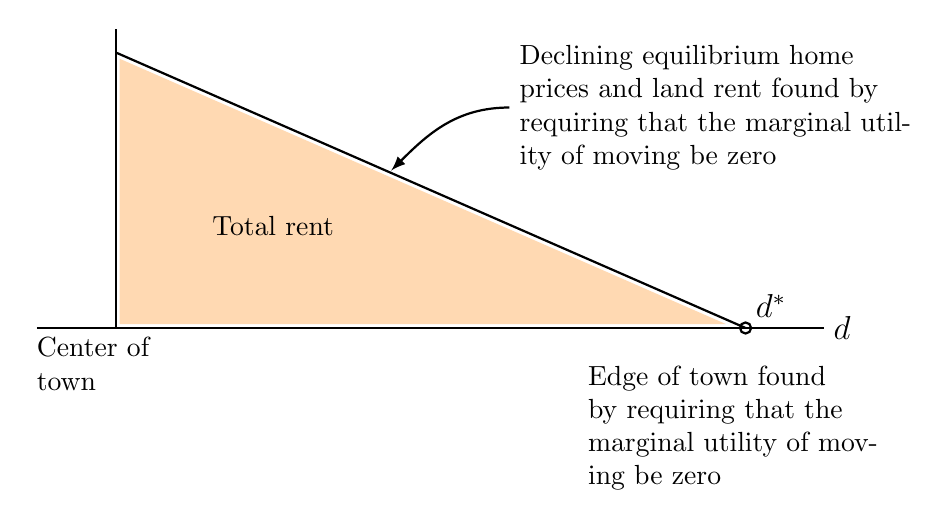
\begin{tikzpicture}[domain=0:2]
%\draw[thick,color=gray,step=.5cm, dashed] (-0.5,-.5) grid (3,3);
\draw[line width=.01] (0,0) -- (10,0) node[right] {\large $d$};
\node at (1,0) [below,text width=2cm] {Center of town};
%\draw[thick ] (0,3)node[above right] {merchant's price in town} -- (10,3) ;
\draw[thick ] (0,0)  -- (10,0); 
\draw[thick, -latex] (6,2.8)
node[right, text width=5cm]{Declining equilibrium  home prices and land rent found by requiring that the marginal utility of moving be zero} 
to [out=180, in=45](4.5,2); 

\fill[orange!30] (1.05,0.05)--(8.75,0.05)--(1.05,3.42)--cycle;

\draw[thick ] (1,0) -- (1,3.8);
\draw[thick ] (9,0)node [above right]{\large $d^*$}circle[radius=2pt] node[below=.35cm,text width=4cm] {Edge of town found by requiring that the marginal utility of moving be zero} -- (1,3.5) ;

\node at (3,1.3){Total rent};
\end{tikzpicture} 
\caption{Illustrating marginal and infra-marginal quantities with the bid-rent curve and aggregate rent.}
\label{fig-land-rent-as-inframarginal}
\end{figure}


In Figure~\ref{fig-land-rent-as-inframarginal}, The level of rent is determined at any distance by individuals making comparison locally. At point $d^*$ the person at the edge of the city decides whether to work in the centre or in the non-urban space. These are \gls{marginal} decisions. The orange area represents  the total rents generated between $d=0$ and $d=d^*$. It is a summation of \textbf{\gls{inframarginal}} rents. Like Ricardo in his classic study \cite{ricardoEssayInfluenceLow1815}, we are concerned with the distribution of rents, which are an  inframaginal quantity.


% \section{SORT}
% providing tractable models.  equilibrium analysis of marginal effects, and representative agents which hid distributional effects, as well as spaceless economic models of markets made it difficult to capture the richer spacial dynamics of urban rents, and the details of the ways economic forces play out for individual actors.

% First they've not tended to build in, in a sophisticated way classical economic theory,
% In general, classical economic theory has not been developed in agent-based modeling work
% Agent-based models have begun with simple models, using and relaxing neoclassical assumptions, and building from first principles. This is absolutely the place to start. As the field matures, it makes sense to introduce theory in a more nuanced way, that connects with classical theory/the history of thought, etc

% Second, relatively little agent-based modelling work integrates with the neoclassical economic work in a way that makes the relation clear/holds the advantages. ABM work tends to both reject neoclassical approaches and rely on neoclassical assumptions.
% More generally only a few agent models (e.g. spruce budworm) connect the analytic and agent models in a clear rigorous way. We focus on holding in addition to the relation with classical theory, a close connection with the many advances made withing neoclassical modelling

% - this connection will make it easier to incorporate in teaching and for mainstream economists to engage on and build with.

% This work builds, first, a simple conceptually clear model tightly integrated with the core economic modelling traditions, that builds on the theory of rent.

% ALSO (Agent modelling also tents to model individuals- we also take some steps to agent-based modelling beyond the individual, and to the work developing model in a mode ideas)

% Third, econ lacks resilience analysis and models, yet hysteresis clearly present in the relation between the built environment and econ activity. Although there's been work on dynamics and individual effects, there has been little work looking at the resilience dynamics in economic models, we take that approach looking at the resilience of community and individual wealth, and the relationship between that wealth and productivity. 

% - This puts resilience dynamics at the center of economic analysis.

% The resilience analysis looks at the dynamics of rent in economic boom and bust cycles.
% There is a ratchet effect, achieved through hysteresis in the system, in which sucks wealth out of communities on the way up and on the way down. % DETAIL ONCE DRAFTED.


% \section{Other notes - to sort}

% % TEMP - here are some other notes we may want to reference or bring in. [[non individualistic modeling of agents]] [[generalizability in agent vs classical econ models]]

% The emphasis is on clarity and connecting with the equilibrium in economics, and systematically relaxing each, to connect with the analytic tradition of economic modelling
% The clarity of intuition of the neoclassical tradition with the deeper root of distribution theory rooted in classical economics and the breath and rigor possible with new tools from the study of complexity and statistical physics.

% Methodological questions: 

%     - agent models (integrating theory more completely into agent models)
    
%     - rent theory

% Core model

%     - static version
    
%     - dynamic version

% Simulations
% Result - hysteresis,
% Policy





% TODO Rename file/label as an appendix, or fill out and make into a chapter again
% In addition to the core contribution linking housing and productivity, there are three methodological lines of contribution, and there are policy implications SUMMARIZE METHODOLOGICAL CONTRIBUTIONS %(rent is key to financialization, however the main urban models don't observe the distribution of rents)


% \subsection{Systems design engineering and the systems level effects of financialization}
% Appropriate for systems design engineering
% - engineering is science to responsibility.

% \section{Political economy}

% early stocks, company run an army to take over land and claim surplus in India- more in line with military/state conquests
% then that translates into the industrial economy
% the notion that productivity came from industrial productivity or human capacity.

% what's question, what went before - politics and economics. department of political economy into the 1960s- politics and older ideas.

% Coarse graining, the scale problem.
% Cross scale modelling, models as library components, fall down and rise up wiwth scales
% Building blocks as toys to play and think with - simple enough assumptions to build with








% \textbf{the french engineers} - method math and back \dots

% econ a kind of reactionary precursor to complex systems.  Adam smith- methodological evolution. ABM and link model.

% not an exercise in modelling, it's an exercise in understanding what's happening
% want to know what's happening in society and what we can do. why we want to talk about hysteresis and the effects on social classes.

% haven't formulated even the theoretical model
% rent and social class not in the Alonso model
% couldn't track whose in what class when you do your analysis of scaling
% large gap but hard to see since not maped, theoretical objects barely formulated.

% DISCOVERY PROCESS
% An accident that we found this model, looking for someone to have answered this, planned to just use economic theory.

% thought the model \dots 

% - to move with the dynamism of how people think. 

% (personal ethnography, co-creation, activist method from australi.)

% Simple agent based modes
% TO DO THIS -
% having done this rockefeller work-- wanted to move between omdels way people thing.

% core decsions fast \dots
% get good results and hold core details in their head \dots

% lots of great models out there. 

% \textbf{Coarse graining, curse of dimensionality}
% flow between these classes of models.

% WE DO THIS
% Link agent based and analytic models.

% conceputally clear modelling traditon not connected to one that lets you look at individual trajectoreis---

% - distribution, a farm, unemployed youth \dots bring in infrastructure from well defined simplified models

% abm is in some ways simpler- this agent does this. 
% -- get input asking someone questions- this is wha t people knwo - do this as a buyer \dots ive assempled these piece \dots

% (we've made it a well formed question by making it a model structure. accepted the conventional knowlege about he large scale dynamics \dots
% formulated the conventional knowleges so it can talk to the input \dots )


% -wasn't clear why we couldn't get what we needed from econ.
% did a bunch of work building a biger model, lots of discusion about the \gls{transmission mechanism}.
% We realized it shoudl be coarse grained. 

% REPRHASE METHODOLOGICAL CONNTRIBUTIONS FROM INTRO

% A MEANS IS USE OF THE 
% Constructing an urban \gls{agent-based model} that is consistent with {neoclassical growth theory}. We show how the neoclassical framework can be implemented in the agent-based framework, and make a case for the usefulness of the approach in linking urban rents and productivity. %Chapter~\ref{chapter-methodology} discuses methodological implications of this approach.

% THIS HAS IMPLICATIONS
% Building a model that is easily extended to explore a range of issues, and used to evaluate policy options. 
% The model combines clear and explicit theoretical assumptions with careful and transparent implementation of the logic. % in code \dots %flexible Python code.
%     % \item Providing a model that we believe
% We have taken care to allow for  both theoretical and policy-relevant extensions in the simulation,  building a base model that aims to be as simple as something like Alonso's urban model \cite{alonsoLocationLandUse1964}, but 
% % To be useful in policy discussions, a model must  
% simulates the relevant system features and can incorporate a range of intervention types. %way the simulation model is coded. 


% IT LETS YOU DO THINGS THAT HAVE BEEN HARD
% - e.g. have tractible models that let you explore \textbf{hysteresis, reversibility}- hopefully bringing it towards the core of analysis
% Resilience.

% DOING THIS IN AN ENGINEERING DEPARTMENT
% Engineering  knowledge for responsibility - just like a bridge, a social choice to have a middle class.
% have housing for everyone, have food for everyone

% social engineering has been a sensitive point- efforts have tended to control.
% Particularly after WWII social experiments, that were horors.

% even building predictive modes is a problem. any intervention that makes your model predictive increases your control.

% Reductionism had some holdouts but largely unchallenged

% %Challenges to reductionism deep within the field too

% Answer is of course to relinquish commitment to state. 

% - syxtems and resilience give  a bridge
% What is the systems compenent - design for the properties- 
% clearly a system

% social engineering- a note on the approach to engineering in social system
% cannot know much about state- have to comite to regime, it is then possible to comit to things like freedom \dots
% to autonomy, relinquish comitent to stat


% RESILIENCE IS CENTRAL TO THE ADVANCE - TO ACTUALLY MAKING AN ENGINEERING OF THE SOCIAL POSSIBLE.


% at the level of capturing and sharing details.

% applied work


% has to do with Social innovation, how societies are transformed,
% gives an ease in relating the model with the action. 

% action and choice
% weak links in hosting, 

% did these models for rockefeller, for the labes-- had a group
% worked iwith the games intstitued ith design \dots




\section{Models in Labs}

Models can act as a boundary object, letting people with different perspectives communicate and build understanding within a system.

1. Where the uncertainty, disputed values, and high stakes, and the decisions that must be made are urgent, the field of study is often referred to as \textbf{post-normal science}. While many different disciplinary and non-academic perspectives are needed here, bringing people together is often difficult and necessitates the development of shared languages that people working in the problem area can use to communicate with each other.
 
2. To help develop these shared languages, design can be used to facilitate communication. Design thinking is embedded throughout lab processes in both the work conducted by researchers and the workshops that bring together participants to build small-scale prototype interventions. In our view, the prototypes themselves are \textbf{‘boundary objects’} that enable people from different perspectives to communicate with each other easily. It is in the reduced cost of communication, not in producing preliminary interventions, that prototypes have their primary impact.

3. These reduced communication costs enable participants to coordinate activities with each other. Sometimes these coordinated activities will include most participants in a common strategy, though this is not the primary goal. Instead, overlapping subsets of participants, often simply pairs, can use the opportunities created by the lab process to build joint projects or to engage in exchange with each other. These new agreements between participants add value and help build capacity for innovation and adaptation in the problem space.


"For example, the \textbf{developmental impact investing approach} argues that using deep knowledge of a complex social-ecological system like affordable housing to guide impact investment can not only lead to more effective impact investments, it can also build a better understanding of the system that impact investors are working to change. This generates a virtuous cycle that can build multidirectional \textbf{pathways to scaling} social innovation (Geobey, Westley, Weber, 2012).